\begin{exercício}{}{exercício9}
    \begin{center}
        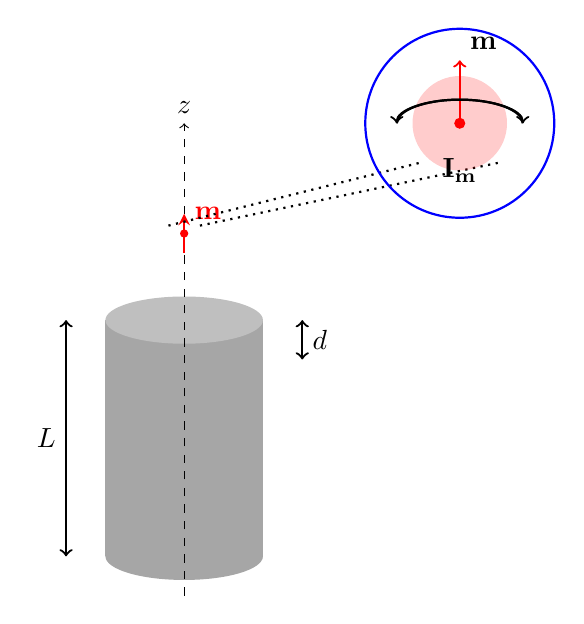
\begin{tikzpicture}
            % Cylinder
            \fill[gray!70] (-1,-3) rectangle (1,0); % Cylinder side
            \fill[gray!50] (0,0) ellipse (1 and 0.3); % Top ellipse
            \fill[gray!70] (0,-3) ellipse (1 and 0.3); % Bottom ellipse

            % Dimension L
            \draw[<->, thick] (-1.5,0) -- (-1.5,-3) node[midway,left] {\(L\)};

            % Dimension d
            \draw[<->, thick] (1.5,-0.5) -- (1.5,0) node[midway,right] {\(d\)};

            % z axis
            \draw[->, dashed] (0,-3.5) -- (0,2.5) node[above] {$z$};

            % Magnetic moment vector m
            \fill[red] (0,1.1) circle (1.5pt);
            \draw[-stealth, thick, red] (0,0.85) -- (0,1.35) node[right] {\textbf{m}};

            % Zoom lines to indicate enlargement
            \draw[dotted, thick] (0.2,1.2) -- (4,2);
            \draw[dotted, thick] (-0.2,1.2) -- (3,2);

            % Zoomed-in circle (zoom view)
            \begin{scope}[shift={(3.5,2.5)}, scale=1]
                % Outer circle for the zoomed view
                \draw[thick, blue] (0,0) circle (1.2);

                % Red shaded circular area in the background
                \fill[red, opacity=0.2] (0,0) circle (0.6);

                % Magnetic moment vector m
                \fill[red] (0,0) circle (2pt); % Central point of the magnetic moment
                \draw[->, thick, red] (0,0) -- (0,0.8) node[above right, black] {\textbf{m}};

                % Elliptical path for current I_m with directional arrows
                \draw[->, thick] (-0.8,0) arc[start angle=180, end angle=0, x radius=0.8, y radius=0.3];
                \draw[->, thick] (0.8,0) arc[start angle=0, end angle=180, x radius=0.8, y radius=0.3];

                % Label for current I_m
                \node at (0,-0.6) {\(\mathbf{I_m}\)};
            \end{scope}

        \end{tikzpicture}
    \end{center}

\end{exercício}
\begin{proof}[Resolução]
\end{proof}
